\def\etal{{\it et al.\/}}

\section{HPS Performance Studies}

We use the HPS detector simulation system based on SLAC's org.lcsim infrastructure for full GEANT4
simulation of the passage and interaction of charged and neutral particles through the SVT 
and the ECal to the muon detector. In the SVT, it creates realistic energy deposits in the silicon 
microstrip detectors, accounts for dead material, simulates APV25 signal sampling every 25 ns, 
creates clusters, and peforms track finding and reconstruction.
In the ECal, the geometry for the flange and vaccum chamber is based on a tessellated 
represantation imported directly from the CAD drawings. It creates energy deposits in individual 
trapezoidal-shape $PbWO_4$ crystals, simulates FADC signal time evolution and sampling every 4 ns, and 
generates triggers based on the  FPGA trigger algorithm implementation.
To maintain the chicane beamline configuration, the field strength of the
chicane magnets must scale with the beam energy. The performance studies were 
made using the field strength of the 
analyzing magnet of 0.25 Tesla at 1.1 GeV, 0.5 Tesla at 2.2 GeV, and 
1.5 Tesla at 6.6 GeV.
Figure  \ref{fig:lcsim} shows a lcsim rendering of the HPS detector.

\begin{figure}[h]
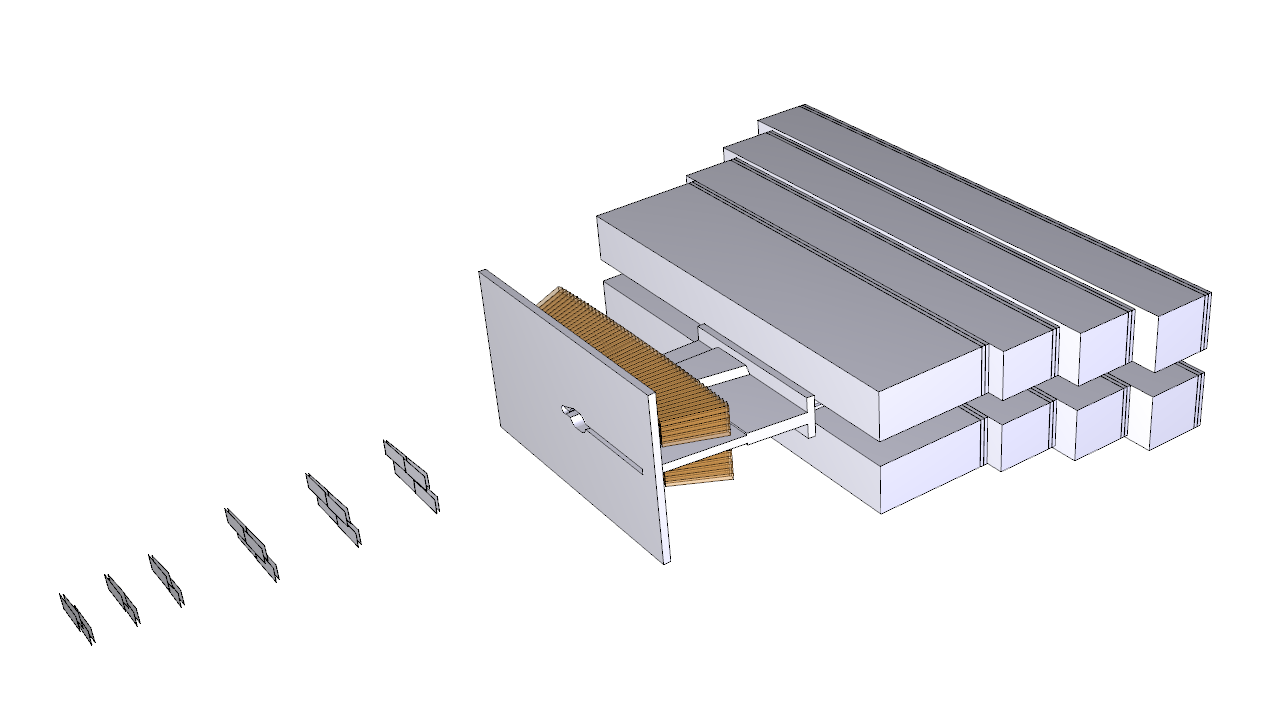
\includegraphics[width=\textwidth]{performance/lcsimDetector}
\caption{\small{ Rendering of the HPS detector simulation}}
\label{fig:lcsim}
\end{figure}

\subsection{Simulation of backgrounds and detector occupancies}

\subsubsection{Simulation of backgrounds}

The multiple Coulomb scattering and bremsstrahlung processes in the target will generate high 
intensity fluxes of electrons and photons in the very forward direction, while the large
M{\o}ller interaction cross section with atomic electrons will generate high intensity low energy
electrons. We use the high energy interaction simulation tools GEANT4 and EGS5 to simulate 
these backgrounds. In the original HPS proposal to JLab PAC37, we described a siginificant 
disageement beween these tools. GEANT4 predicted a broader angular
distribution of multiple scattered electrons than EGS5, resulting in twice the occupancy in the
tracker near the dead zone and much higher ECal trigger rates. 
To resolve this disagreement, we proposed a test run, and the outcome of the test run is described 
in the previous section. The algorithms used 
in the codes to simulate the multiple scattering have been studied, and the findings are summarized in
Appendix. The test run result and the algorithm studies have concluded that EGS5 can describe the multiple scattering 
tails more correctly than GEANT4. All the electromagnetic interactions in the target are simulated using EGS5.   

When bound electrons in the target are ionized by incoming electrons or secondary photons, outer 
shell electron will fill the vacancy and characteristic X-rays are emitted. 
These X-rays can contribute background hits in
the SVT when a conversion takes place in the silicon sensors via the photoelectric effect 
or pair productioncon. While the X-ray production is simulated in EGS5, the X-ray intensity at SVT layer 1
can be estimated using  the impact ionization 
cross section, $\sigma_I$, \cite{hoffmann}, the fluorescence yield, $\omega$, \cite{hubbell},
the photoabsorption length in Tungsten, $\lambda_W$, to account for the self-absorption, and the solid 
angle of the SVT layer 1.
Table \ref{tab:xray} summarizes these parameters and the expected X-ray
fluxes at SVT Layer 1 for 0.25\% $X_0$ Tungsten and 100 nA beam current in 8 nsec time window. 

\begin{table}[h]
\begin{center}
\begin{tabular}{|c|c|c|c|c|c|} \hline
  & Energy (keV) & $\sigma_I$ (barns) & \hspace{0.5 cm} $\omega$ \hspace{0.5 cm} & $\lambda_W$ ($\mu$m) & $N_\gamma$ at Layer 1 in 8 ns   \\ \hline
K-shell & 60 & 40 & 0.95 & 100 & 0.5 \\ \hline
L-shell  & 10 & 1000 & 0.30 & 5 & 2 \\ \hline
M-shell  & 2 & 20000 & 0.02 & 0.2 & 0.1 \\ \hline
\end{tabular}
\end{center}
\caption{\small{X-ray intensities}}
\label{tab:xray}
\end{table}

Hadrons are also produced in the target. The hadron production is at least three order
of magnitude smaller than the electromagnic interaction. The polar angle of the hadron productions
is predominantly at larger than 100 mrad, whereas the HPS detector acceptance is limitted to less than
100 mrad. Furthermore, the hadron energy spectrum is soft as they are produced from the 1/k bremsstrahlung
spectrum and more than 90\% of the hadrons are swept away by the analysing magnet before reaching the ECal.
 The hadron production is simulated using GEANT4 and FLUKA. In the target thinner than
about 5\% $X_0$, the ``virtual'' photon interaction is dominant. \cite{mohring} The inclusive hadron
production ${\sigma (eA\rightarrow X)}$ is simulated from the photonuclear process ${\sigma (\gamma A
\rightarrow X)}$ using the equivalent photon approximation,

$$ \sigma (eA \rightarrow X) = \int \sigma_k(\gamma A \rightarrow X) dn(k), $$

\noindent
where $dn(k)$ is the number of equivalent photons with energy $k$ \cite{budnev} and there are 
approximately $8 \times 10^{10} $ photons in 6.6 GeV 100 nA beam. 
Table \ref{tab:pion} summarizes the pion single rates from 1\% $X_0$ Tungsten target
and 6.6 GeV 100 nA beam. While the pion production is higher in GEANT4, the energy spectrum is softer and
consequently the single rate of pions reaching the ECal is lower in GEANT4. While the pions look like a minimum 
ionizing particle in the ECal most of the time, they can deposit a significant energy when ${\pi^0}$ are
produced in the ECal crystals, and together with the beam background, they contribute accidental coincident triggers. 

\begin{table}[h]
\begin{center}
\begin{tabular}{|c|c|c|} \hline
  & Total production rate (kHz) & Single rate reaching the ECal (kHz) \\ \hline
GEANT4 & 410 & 8 \\ \hline
FLUKA  & 240 & 15 \\ \hline
\end{tabular}
\end{center}
\caption{\small{Pion single rates from 1\% $X_0$ Tungsten target at 6.6 GeV 100 nA}}
\label{tab:pion}
\end{table}

\pagebreak
\noindent
Other beam induced background we considered are:

\begin{itemize}
\item
Beam halo

Beam halo was measured using a large dynamic range halo monitor during the 6 GeV era. The beam halo 
that extends to 2 mm was found at the level of $10^{-7}$. At this level, the halo contribution in 
the SVT occupancy is negligible. It is expected that behavior of the 12 GeV machine will be
understood at the same level.

\item
Synchrotron radiations

Synchrotron radiations are produced from the last dipole magnet in the beam line in the vertical 
plane, and from the chicane magnets in the horizontal plane. Since the characteristic energy is 
proportional to $E_{beam}^2$, synchroton radiations are of concern 
only at 6.6 GeV. The characteristic energy ($k_c$),
the average energy ($k_{ave}$), and the power of synchrotron radiations are summarized in 
Table \ref{tab:sync}.
None of the radiations from the last dipole will enter the HPS detector as the radiations will be intersected 
by the beamline collimator. The radiations from the chicane magnets are in the dead zone, and
none of the detector components are designed to intersect the beam plane.   

\begin{table}[h]
\begin{center}
\begin{tabular}{|l|c|c|c|c|} \hline
  Source & $k_c$ (keV) & $k_{ave}$ (keV) & $N_\gamma$ per e- & Power (mW) at 100 nA \\ \hline
  virtical bend & 19 & 5.9 & 4.0 & 2.4 \\ \hline
  Frascati Magnet & 52 & 16 & 4.6 & 7.4 \\ \hline
  PS magnet   & 44 & 14 & 9.3 & 13 \\ \hline
\end{tabular}
\end{center}
\caption{\small{Synchrotron radiations at 6.6 GeV}}
\label{tab:sync}
\end{table}


\item
EM induced backgrounds

Electromagnetic fields induced by the high intensity beam could interfere with the SVT and its electronics
as the detector is located as close as 0.5 mm from the beam. We have evaluated the direct beam field and its wake 
field, the diffraction radiations from the beamline apertures, and the transition radiations from
the target. The intensities of these EM induced backgrounds are small and no interferance with the SVT
is expected.
 
\end{itemize}

\subsubsection{Simulated Tracker Occupancies}

Figure \ref{fig:scatt} shows the distribution of charged particle hits in Si tracker layer 1 
which is located 
10 cm from the target. The beam energy is 6.6 GeV, and the target thickness is 
0.25\% $X_0$. Multiple Coulomb scattered beam electrons are confined within 0.5 cm of the beam axis
(x=y=0), while the low energy M{\o}ller electrons are distributed in a parabolic shape. There are
very few positrons. From these distributions, the detector occupancy in the horizontal Si strip
sensor in the 8 ns time window is calculated for a 400 nA beam current and five different target
thicknesses, 1.0\% $X_0$, 0.5\% $X_0$, 0.25\% $X_0$, 0.1\% $X_0$, and 0.05\% $X_0$, and is shown
in Figure \ref{fig:occup}. As described in Section xx, the dead zone is defined by using 
a criterion that the
maximum occupancy in Layer 1 is 1\%. For a 0.25\% $X_0$ target and 430 nA beam, the occupancy is 
1\% at a distance of 1.5mm from the beam in Layer 1, which corresponds to a dead zone of $\pm$ 15
mrad. As long as the product of target thickness (T) and beam current (I) is constant, the same 
$A'$ production rate is maintained. Since the multiple scattering and hence the effective beam size 
is reduced in a thinner target, it is advantageous to use a thinner target and a higher current.
Using the constraint that the occupancy is 1\% at 15 mrad, we find the beam current $I$ which 
gives this occupancy for each of several potential target thicknesses $T$. The quantity 
$(I\cdot T)^{1/2}$, which is approximately proportional to the sensitivity $S/\sqrt{B}$, is
given in Table \ref{tab:occup}, showing how the sensitivity improves as the target thickness 
decreases.

\begin{figure}[h]
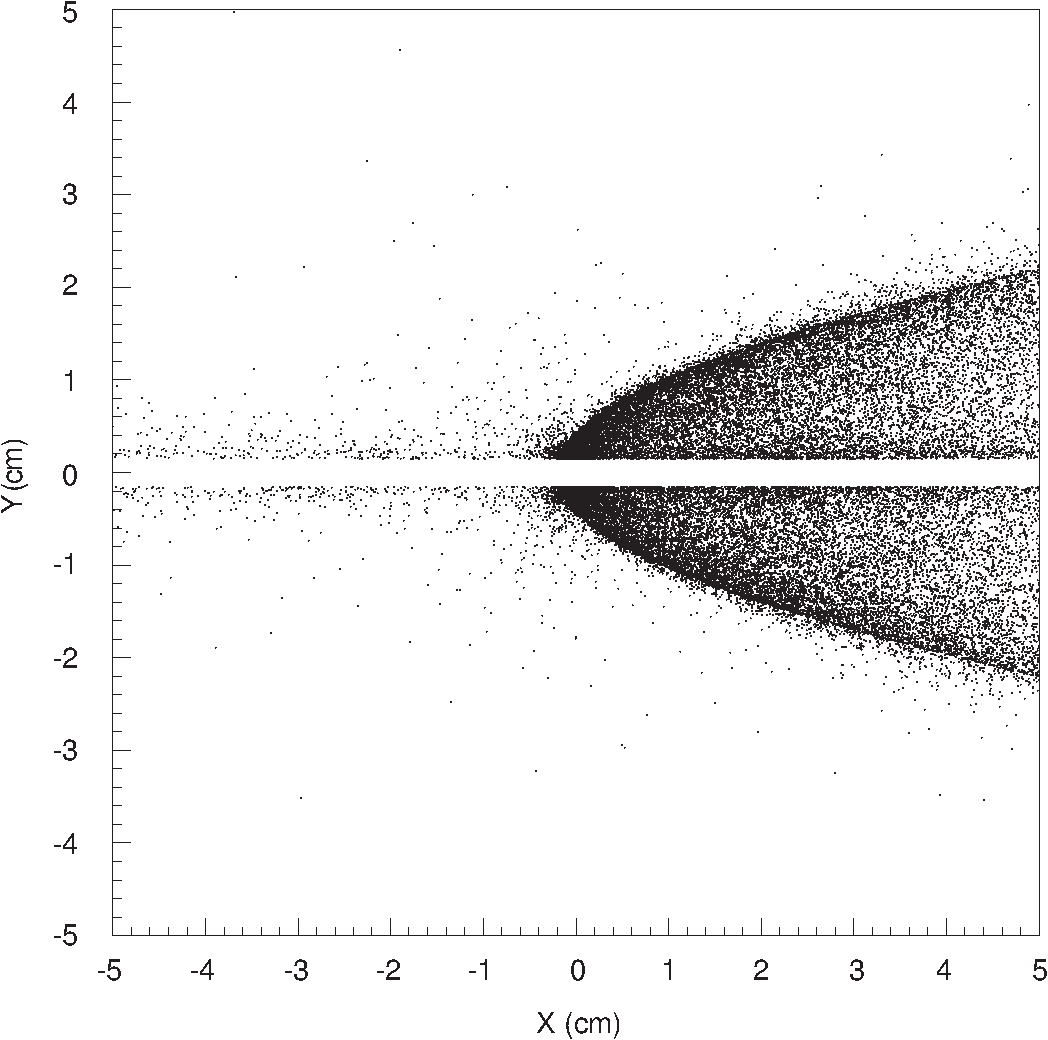
\includegraphics[width= 4 in]{performance/scatterplot.pdf}
\caption{\small{Charged particle distribution in SVT layer 1.}}
\label{fig:scatt}
\end{figure}

\begin{figure}[t]
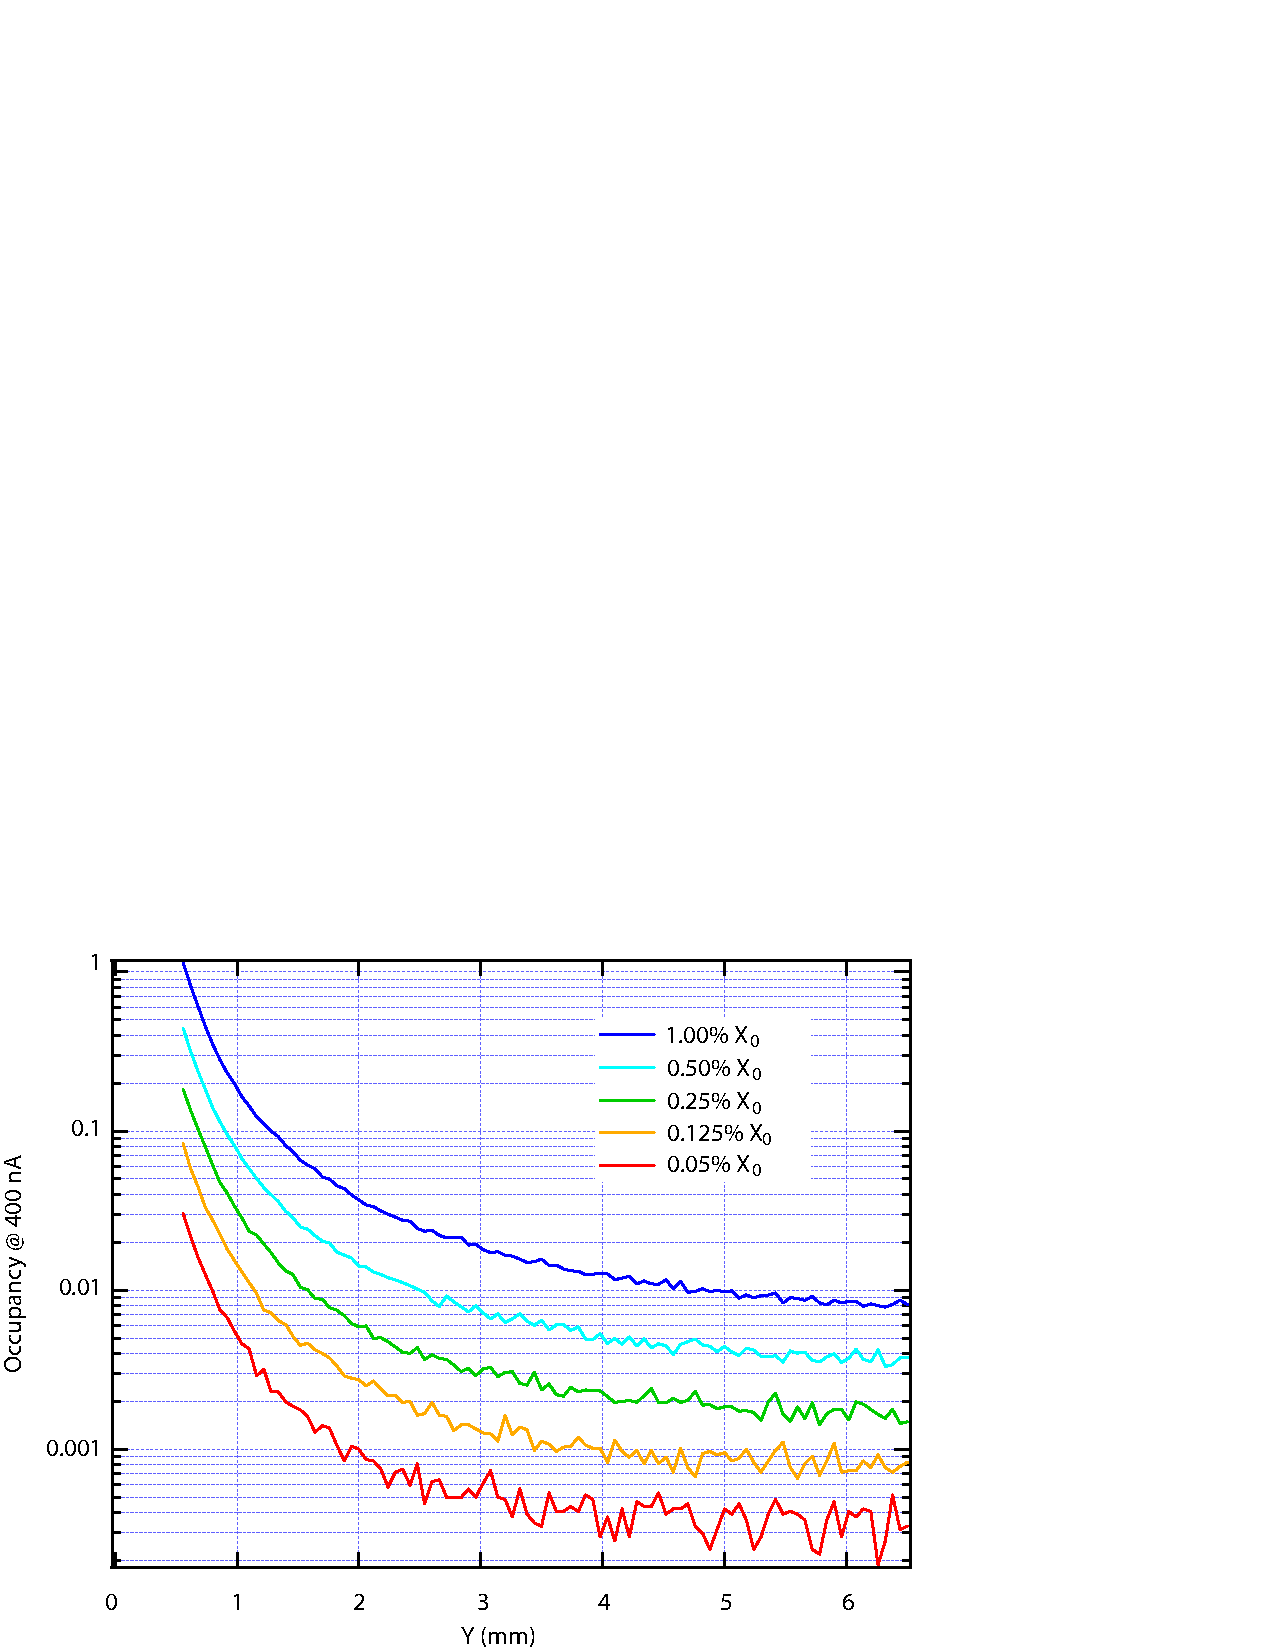
\includegraphics[width=\textwidth]{performance/occupancy.pdf}
\caption{\small{Sillicon sensor layer 1 occupancy at 400 nA vs. distance from the
beam in mm.}}
\label{fig:occup}
\end{figure}

\begin{table}[h]
\begin{center}
\begin{tabular}{|c|c|c|} \hline
  Target thickness (\% $X_0$) & Beam Current (nA) & $\propto S/\sqrt{B}$ \\ \hline
  1.0 & 60 & 7.7 \\ \hline
  0.5 & 170 & 9.1 \\ \hline
  0.25 & 430 & 10.4 \\ \hline
  0.10 & 1330 & 11.6 \\ \hline
  0.05 & 2860 & 11.9 \\ \hline
\end{tabular}
\end{center}
\caption{\small{Beam current yielding 1\% occupancy in SVT layer 1 for various target 
thicknesses at 6.6 GeV, and the relative experimental sensitivities which result.}}
\label{tab:occup}
\end{table}

The run conditions for other possible beam energies are studied using the same criterion that the maximum occupancy 
in SVT Layer 1 does not exceed 1\%. Table \ref{tab:runc} summarizes the target thickness and proposed beam current. 

\begin{table}[h]
\begin{center}
\begin{tabular}{|c|c|c|} \hline
  Beam Energy & Target thickness (\% $X_0$) & Beam Current (nA) \\ \hline
  1.1 & 0.125 & 50 \\ \hline
  2.2 & 0.125 & 200 \\ \hline
  4.4 & 0.25  & 300 \\ \hline
  6.6 & 0.25 & 450 \\ \hline
\end{tabular}
\end{center}
\caption{\small{Run Conditions}}
\label{tab:runc}
\end{table}

\subsubsection{Simulated ECal Occupancies}

There are two factors limiting the allowable ECal occupancy. First, the ECal 
readout algorithm uses a window of fixed size to integrate hit energy. This 
window was set to 140 ns ($35 \times 4$ ns) for the test run, and so the 
number of hits above readout threshold in a 140-ns time window should be well 
below 1. Figure \ref{fig:ecal_rate} shows that the maximum rate in any crystal 
is 500 kHz, which translates to 0.07 hits in 140 ns.

Second, because the FADC only reads out on a rising threshold crossing, each 
hit above threshold causes dead time for that crystal until the preamp output 
falls back below threshold. Figure \ref{fig:ecal_deadtime} shows the fraction 
of time each crystal spends above threshold. The maximum dead time is 0.03, 
meaning that even the hottest crystal is sensitive to new hits 97\% of the time.

\begin{figure}[ht]
	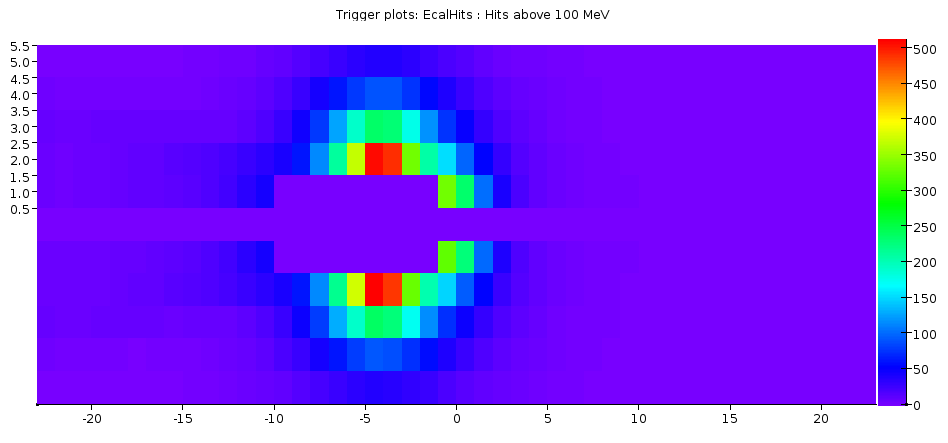
\includegraphics[width=\textwidth]{performance/ecal_rate_100mev_22}

	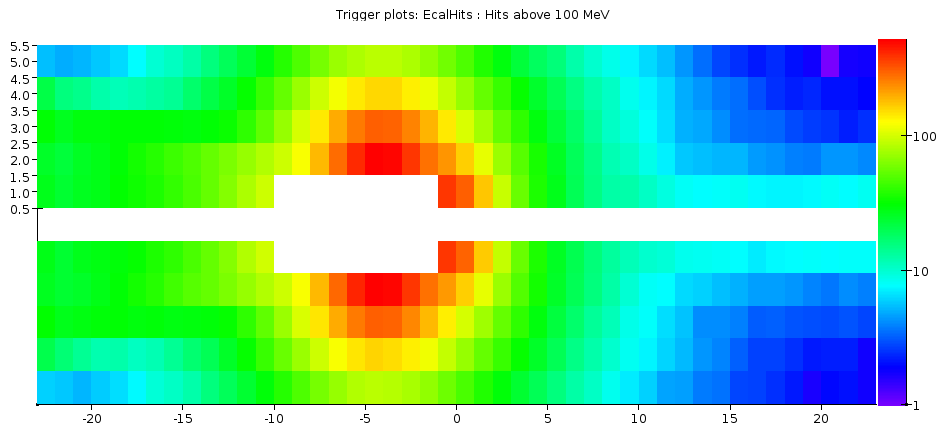
\includegraphics[width=\textwidth]{performance/ecal_rate_100mev_22_log}
	\caption{\small{Rate of hits over 100 MeV (units of kHz) per crystal, 
for 2.2 GeV beam. Top plot uses linear scale for the Z-axis; bottom plot is log scale.}}
	\label{fig:ecal_rate}
\end{figure}

\begin{figure}[ht]
	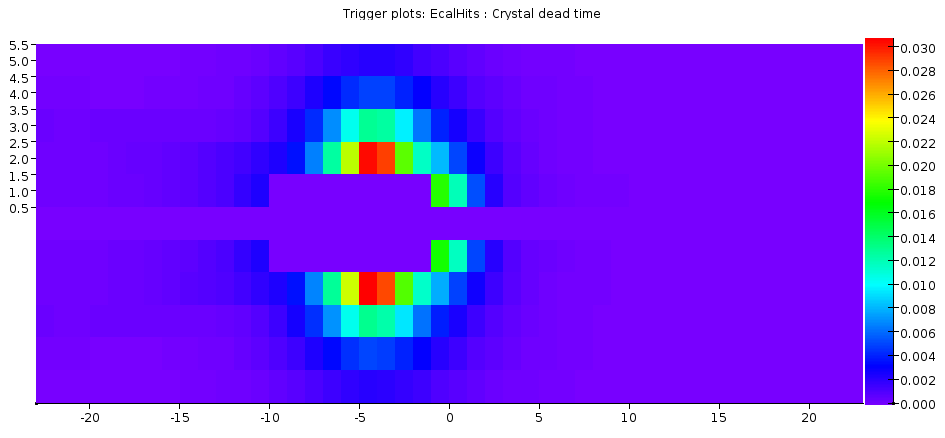
\includegraphics[width=\textwidth]{performance/ecal_deadtime_22}
	\caption{\small{ECal readout deadtime fraction for 2.2 GeV running, 
with a threshold of 75 MeV for each crystal.}}
	\label{fig:ecal_deadtime}
\end{figure}

\subsection{ECal Trigger Performance}

The proposed ECal trigger was simulated to test trigger cuts, verify
that the trigger has acceptable efficiency for A' events, and verify 
that the trigger rate is compatible with the HPS DAQ in all running conditions. 

The complete chain of signal evolution in the ECal crystals and 
signal processing through the trigger system was simulated
by following closely the ECal trigger description in Section xx. 
Starting from the energy deposits in the ECal crystals, signals were 
generated using the CR-RC shaper function with a time constant of 15 ns
measured with the ECal crystals, amplitudes were sampled every 4 ns
and pulse data evaluated every 32 ns (simulating FADC), and the cluster 
finding algorithm and trigger logic were applied (simulating CTP and SSP). 

The CEBAF beam bunch structure was simulated by sending one bunch 
equivalent of electrons, 
625 (1.1 GeV), 2,500 (2.2 GeV) and 5,625 $e^-$'s (6.6 GeV), through 
the target, and total 50 million bunches of beam backgrounds were 
generated at each beam energy. Since the trident production process 
was not in EGS5, trident events were generated with MadGraph/MadEvent 
and overlaid on the beam background bunches with a proper bunch separation 
expected from the trident cross section.
For the trigger acceptance studies, A' events were generated with 
MadGraph/MadEvent at 1.1, 2.2, and 6.6 GeV.

The trigger parameters described in Section \ref{sec:triggerdaq} are 
chosen by running the simulation and plotting the relevant variables 
for beam background and A' events. This is done for each beam energy 
and a set of A' masses for each beam energy. 
Figure \ref{fig:coplanarity} shows the coplanarity angle vs. the azimuthal 
angle of the lower-energy cluster, indicating that A' events 
tend to have small coplanarity angles. Figure \ref{fig:energy-distance} shows
the distance from beam axis vs. energy of the lower-energy cluster,
indicating that the energy-distant cut can reduce the beam background effectively.
Figure \ref{fig:ediff} shows the cluster energy difference vs. energy sum,
indicating that the energy sum cut can retain A' events effectively.       

\begin{figure}[ht]
	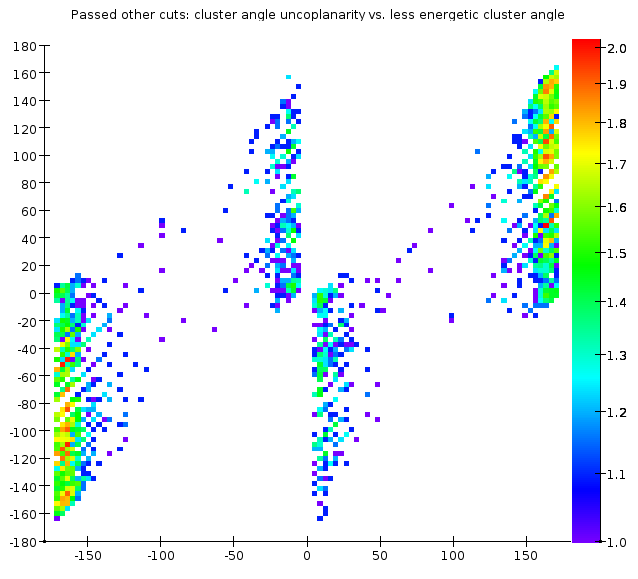
\includegraphics[width=0.4\textwidth]{performance/coplanarity_22}
	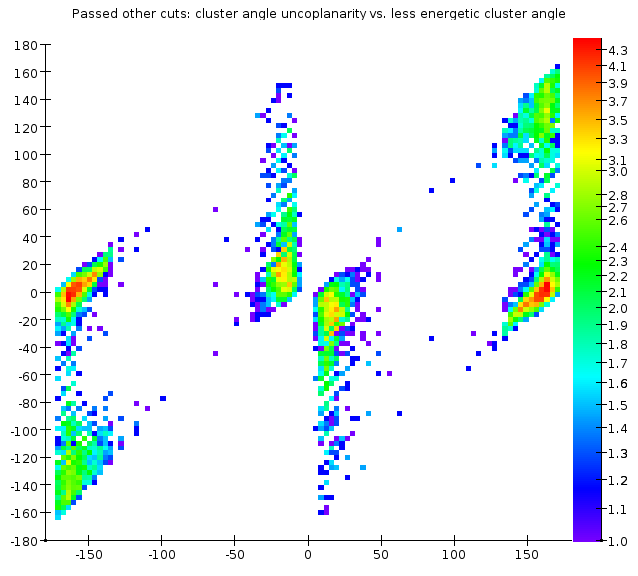
\includegraphics[width=0.4\textwidth]{performance/coplanarity_22_075mev}
	\caption{\small{Deviation of cluster pairs from coplanarity (units of degrees) for 2.2 GeV beam; background and 75 MeV A' tridents are shown.}}
	\label{fig:coplanarity}
\end{figure}

\begin{figure}[ht]
	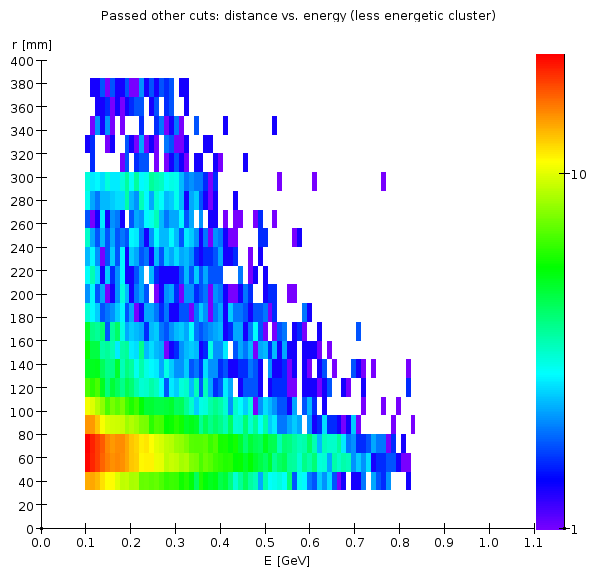
\includegraphics[width=0.4\textwidth]{performance/energy-distance_22}
	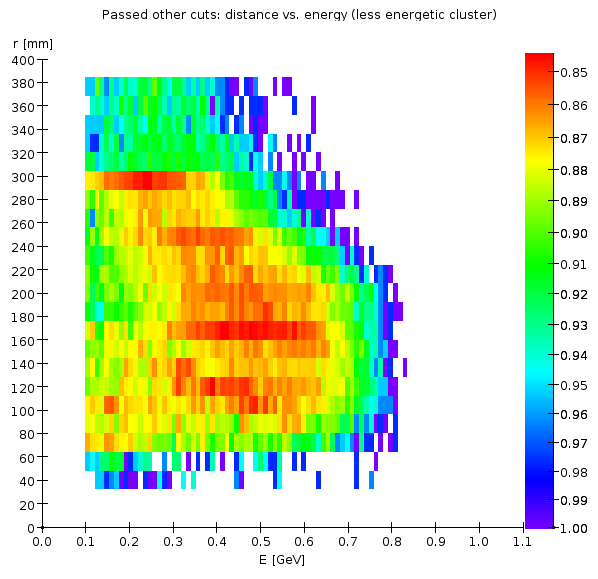
\includegraphics[width=0.4\textwidth]{performance/energy-distance_22_075mev}
	\caption{\small{Energy and distance from beam axis of the lower-energy cluster, for 2.2 GeV beam; background and 75 MeV A' tridents are shown.}}
	\label{fig:energy-distance}
\end{figure}

\begin{figure}[ht]
	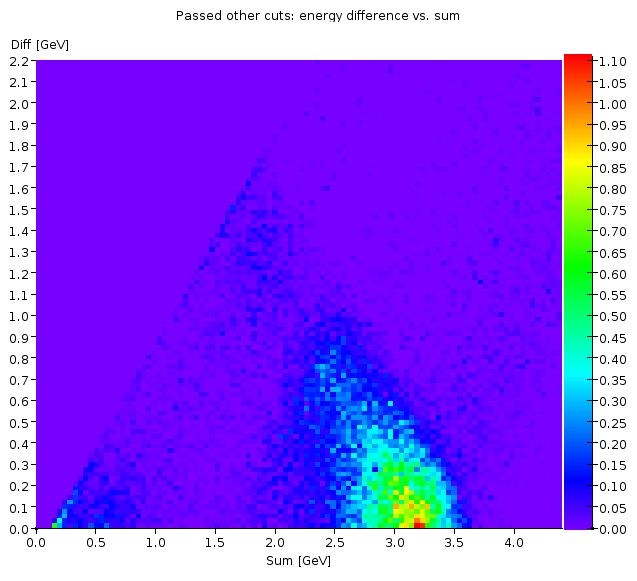
\includegraphics[width=0.4\textwidth]{performance/ediff_22}
	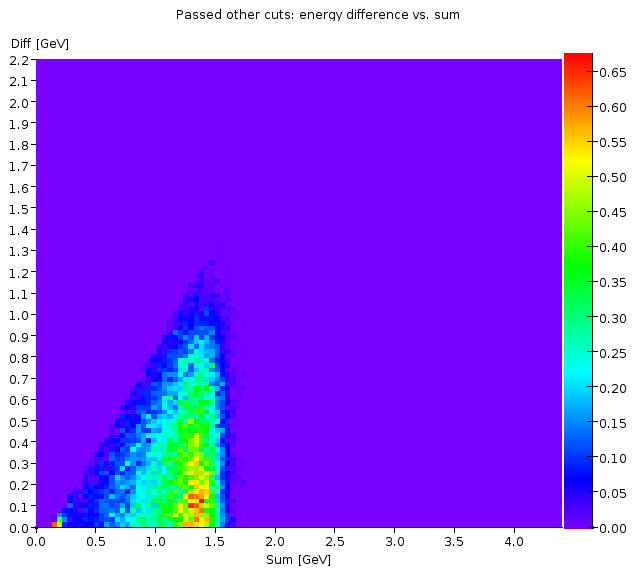
\includegraphics[width=0.4\textwidth]{performance/ediff_22_075mev}
	\caption{\small{Energy sum and difference of cluster pairs, for 2.2 GeV beam; background and 75 MeV A' tridents are shown.}}
	\label{fig:ediff}
\end{figure}

The following trigger parameters were determined to be independent of beam energy:
\begin{itemize}
	\item Minimum cluster energy ($E_{min}$): 0.1 GeV
	\item Distance ($r_{edist}$) in the energy-distance cut: 200 mm
	\item Energy ($E_{edist}$) in the energy-distance cut: $0.5\times E_{beam}$
\end{itemize}

Table \ref{tab:trigcuts} summarizes the trigger parameters that were found dependent on the beam energy. 
The remaining trigger parameters given in Section \ref{sec:triggerdaq} did not have a significant 
effect on specificity of the trigger.

\begin{table}
	\begin{tabular}{|l|r|r|r|}
		\hline
		Beam energy [GeV] & $E_{max}$ [GeV] & $Esum_{max}$ [GeV] & $\Delta\phi_{max}$ [$^\circ$] \\
		\hline
		1.1	&	0.7	&	0.8	&	90\\
		2.2	&	1.6	&	1.7	&	45\\
		6.6	&	5.0	&	5.5	&	60\\
		\hline
	\end{tabular}
	\caption{ {\small Trigger parameters optimized for different beam energies.}
	\label{tab:trigcuts}}
\end{table}

Trigger rates are shown in Table \ref{tab:trigrates}. These rates are safely under the maximum readout rate of 43 kHz set by the SVT DAQ. The uncertainties on the rates are due to the beam background statistics. 
The addition of pions to the 6.6 GeV background sample does not have a significant effect on the trigger rate.

\begin{table}
	\begin{tabular}{|l|r|}
		\hline
		Sample &  Rate (kHz)\\
		\hline
		1.1 GeV	Beam Background 		& 15.7 $\pm$ 0.4	\\
		1.1 GeV Beam Background+tridents	& 17.6 $\pm$ 0.6	\\
		2.2 GeV	Beam Background			& 11.2 $\pm$ 0.3	\\
		2.2 GeV Beam Background+tridents	& 15.8 $\pm$ 0.4	\\
		6.6 GeV	Beam Background			& 10.2 $\pm$ 0.3	\\
		6.6 GeV Beam Background+tridents	& 12.6 $\pm$ 0.4	\\
		%6.6 GeV EGS5+tridents+pions (FLUKA)	& 7.3 $\pm$ 0.3	\\
		%6.6 GeV EGS5+tridents+pions (G4)	& 7.0 $\pm$ 0.3	\\
		\hline
	\end{tabular}
	\caption{ {\small Trigger rates using various background samples. }
	\label{tab:trigrates}}
\end{table}

Trigger efficiency for A' events is defined as the fraction of A' tridents (generated without fiducial cuts) that produce a trigger.
For the performance of the experiment, we are interested in the combined efficiency of the trigger and tracker: the fraction of A' tridents that produce a trigger and leave enough hits in the tracker for a pair of tracks to be reconstructed.
We simulate charge deposition and readout of the tracker (turning off the generation of noise hits), and check each sensor for hits. 
If the DAQ reads out hits in four stereo pairs in each half of the tracker, the event is in the combined acceptance. 
Figure \ref{fig:trigeff} shows the ECal trigger efficiency and the ECal/SVT-combined efficiencies for A' events at 1.1, 2.2, and 6.6 GeV. 
Both trigger and tracker acceptances are dominated by the geometric acceptances of the ECal and tracker.
A' prompt decays are assumed.

\begin{figure}[ht]
	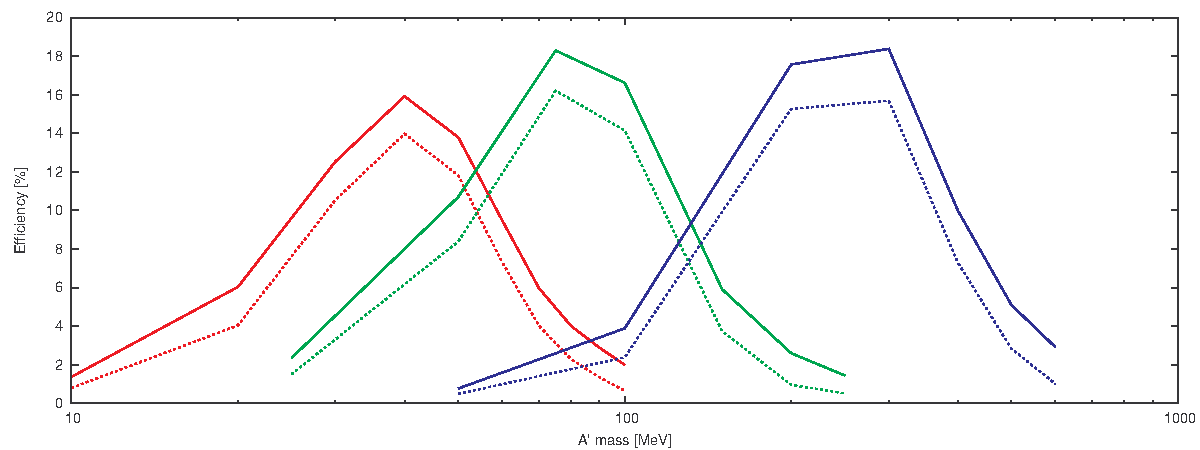
\includegraphics[width=\textwidth]{performance/ap_eff}
	\caption{\small{Trigger efficiency (solid lines) and combined efficiency (dashed lines) as a function of A' mass, at beam energies of 1.1, 2.2 and 6.6 GeV (red, green and blue respectively). A' prompt decays are assumed}}
	\label{fig:trigeff}
\end{figure}


\bibliographystyle{unsrt}
\begin{thebibliography}{99}
\bibitem{hoffmann}
D.H.H. Hoffmann \etal, Z. Physik {\bf A293}, 187 (1979)

\bibitem{hubbell}
J.H. Hubbell \etal, J. Phys. Chem. Ref. Data, Vol. {\bf 23}, 339 (1994) 

\bibitem{mohring} H.-J. M\"{o}hring, Nucl. Instrum. Methods {\bf A292}, 482 (1990)

\bibitem{budnev} Y.M. Budnev \etal, Phys. Rep. {\bf 15C}, 181 (1975)

\end{thebibliography}


